\section{Software Taxonomy --- TODO by 0000 15th August 2013} \label{taxonomy}

In \cite{Woodings2013Tut1}, Woodings displays an example taxonomy in the form of
a decision tree.
We aim to replicate the decision tree hierarchy by noting some interesting
structural and semantic differences between the models and thus be able to
comment on the interesting and salient characteristics of each.\\
\\
We begin by noting that there are ``iterative" and ``non-iterative" models.
But what does this actually mean?
Many of the processes we made in our notation have a ``verification" stage that
iterates within the stage.
``Iterative" and ``non-iterative" are thus too general labels to begin with.\\
\\
Instead, we note that the ``agile" and ``non-agile" methods have two very
different features.
``Agile" methods have feedback from clients and users during the coding stage as
to how the product so far looks.
``Non-agile" methods do not engage in this; they specify requirements at the
beginning, get them as correct as possible, and then continue with the
implementation.\\
\\
We can thus use a first division as {\bf ``does the process have a user-feedback
stage during implementation?"}
This almost neatly divides our set of models in two partitions, $S_{yes}$ and
$S_{no}$ (for ``yes" and ``no" to our answer respectively).
The ``evident" partitions would be
\begin{itemize}
  \item $S_{yes} = \{$ Crystal Clear, Extreme Programming, Evolutionary, Scrum $\}$
  \item $S_{no} = \{$ Waterfall-1, Waterfall-2, Waterfall-3, Spiral, V-Model$\}$
\end{itemize}
There are three interesting cases that are more difficult to classify
\begin{enumerate}
  \item the incremental model is an iterative, semi-agile model that revolves
  around implementing small chunks of work in a waterfall-esque fashion.\\
  \\
  One might argue that a single iteration of waterfall is an implementation stage,
  but we will choose to instead say that the implementation or coding stage of
  the waterfall iteration is the task which needs a user-feedback stage.\\
  \\
  As it does not, we can say that it is belongs in the $S_{no}$ partition.
  \item similarly, test-driven development is another interesting case due to
  its iterative nature.
  However, pure test-driven development does not contain a user-feedback stage,
  and it is a simple methodology to encode a testing mindset into developers.
  As a result, we say that test-driven development also belongs in $S_{no}$.
  \item rapid prototyping does not actually revolove around the implementation
  stage, since it is a special case of requirements gathering.
  Since by our original modelling assumptions, this requirements gathering is
  independent of any other process in the development methodology, rapid
  prototyping does not belong to $S_{no}$ or $S_{yes}$.\\
  \\
  Instead, we create a third partition, $S_{rapid} = \{$ Rapid Prototyping $\}$ which is a singleton set
  containing only rapid prototyping.
\end{enumerate}

So far, we have divided our initial set of models into three possible models.
This is shown in Figure \ref{DecTree1}.

\begin{figure}[ht!]
  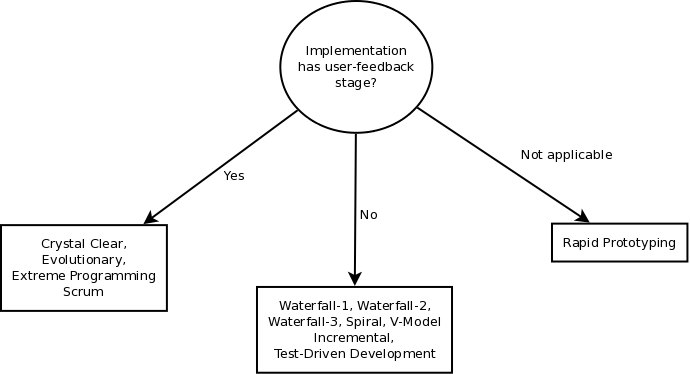
\includegraphics[scale=0.4]{media/DecisionTree1}
  \caption{Our initial decision tree. We can see each of $S_{no}$, $S_{yes}$ and $S_{rapid}$.}
  \label{DecTree1}
\end{figure}

We will focus on subdividing $S_{yes}$.
These are models that are ``agile" in their mannerisms.
We note that out of the four models, two of them involve modifying a project
plan.
The others do not; instead, both Scrum and Evolutionary are feature-driven, with
an intent to ``grow" the project (indeed, we might find they are the same
process by the end!).
We will thus subdivide $S_{yes}$ into two new partitions
\begin{itemize}
  \item $S_{plan} = \{$ Crystal Clear, Extreme Programming $\}$
  \item $S_{grow} = \{$ Scrum, Evolutionary $\}$
\end{itemize}
This labelling reflects some interesting properties of the methods under review.
We note that the two partitions are focused on an organic method of
growing a project, versus a prescribed plan that should be flexible when meeting
user requirements.
Both of these are in the spirit of ``user-feedback" and ``user-focused"
development, but one might have more group might have more foresight and risk
management inbuilt ($S_{plan}$) whilst the other might be more flexible and
reactive ($S_{grow}$).\\
\\
We have achieved a further level of granularity with our second subdivision.
This is shown in Figure \ref{DecTree2}.
\begin{figure}[ht!]
  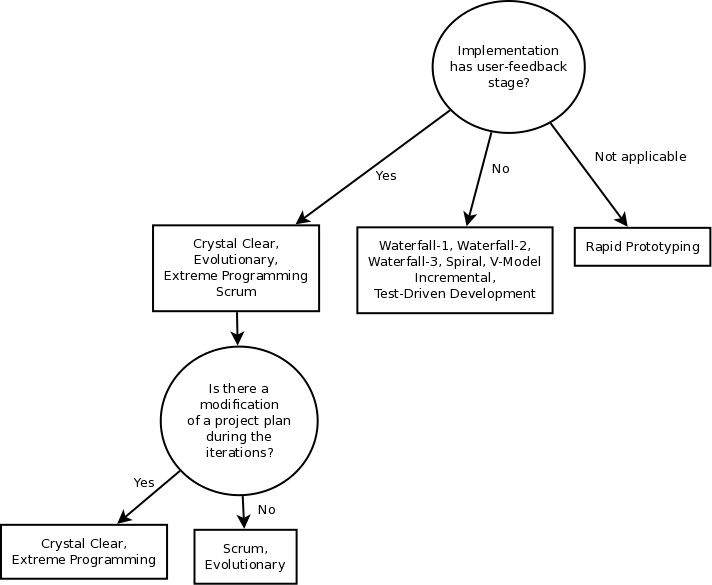
\includegraphics[scale=0.4]{media/DecisionTree2}
  \caption{A second iteration of our decision tree. We have now managed to
  subdivide $S_{yes}$ into sets of size two.}
  \label{DecTree2}
\end{figure}

We now find some interesting results.
When trying to separate Scrum and Evolutionary, it becomes difficult to find
many differences between the two.
Perhaps the only real differences lie in the meanings behind what happens; there
are assigned roles in Scrum for studying and deciding what users want, whereas
Evolutionary does not have as rigid structure in organising the system.
We will use this to differentiate between the two processes, though we note that
this is a small difference and it is hard to justify this as a good
differentiator between the two.\\
\\
To separate Extreme Programming and Crystal Clear, we note that in Figure
\ref{WindowsXP} there is a mandatory requirement of Peer Review and Pair Coding.
The verification process in Crystal Clear does not have nearly so many levels of
verification around coding specified.
Thus, we use the following question as our discriminator: ``are there multiple
levels of verification centred around coding specified in the process?"\\
\\
We should note that the questions at this level are very subjective and are not
as definitive as our previous questions.
As an example, the testing process in Crystal Clear is not specified; a
practitioner could add in multiple feedback loops and thus almost make it
indistinguishable from Extreme Programming.
Thus, in some cases, we could claim that Extreme Programming and Crystal Clear are the
same process, and the same could be said of Scrum and Evolutionary.
Thus, we will use a dotted line to represent a pseudo-``equivalence class" of
processes that are almost the same, except for perhaps some implementation
differences.
Figure \ref{DecTree3} is our first iteration of actual definitive classification
(that is, we can now actually classify some models based on their
characteristics).

\begin{figure}[ht!]
  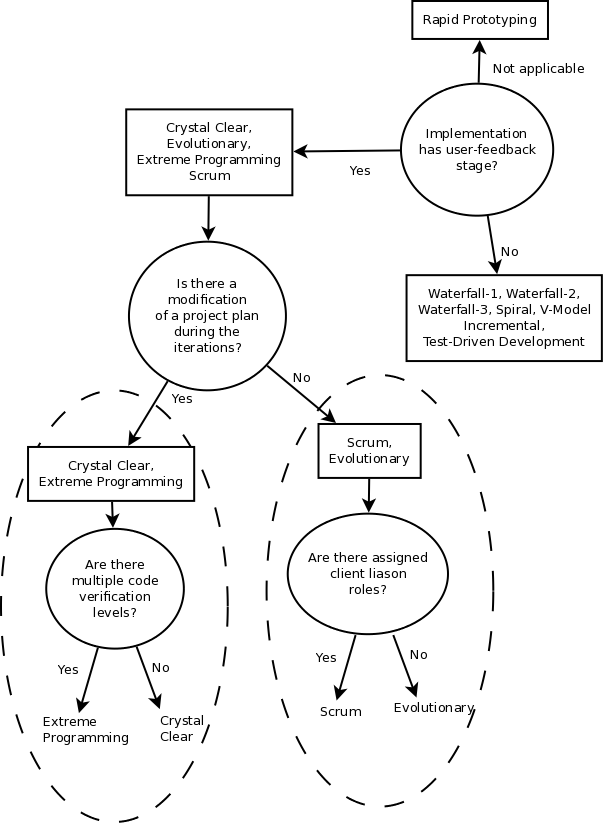
\includegraphics[scale=0.4]{media/DecisionTree3}
  \caption{A third iteration of our decision tree. We can definitively classify
  four of our processes by their structure and semantics, and we use an
  ``equivalence class" to denote models that appear to be the same.}
  \label{DecTree3}
\end{figure}

We now consider the problem of subdividing the much larger class $S_{no}$ into
partitions.
We note the following unique characteristics
\begin{itemize}
  \item Waterfall-1 has no feedback at all
  \item Waterfall-2 and Waterfall-3 have iterations between stages
  \item Test-Driven Development is only a specification of how to write code
  during the implementation stage
  \item Incremental is an iterative loop methodology
  \item Spiral has a risk-assessment stage inbuilt into the project
  \item V-Model specifies all verification plans before the implementation
  begins
\end{itemize}

These are definitive characteristics in our notation and we will use them to
subdivide $S_{no}$.
Of note is that these questions or defining characteristics are in many cases
ambiguous; having a risk-assessment stage is something that could be easily
built into another process, and it is thus difficult to at times distinguish
between models.
Refer to Figure \ref{DecTree4} for our breakdown of models.
For compactness, we only show the subtree of our decision tree that breaks down
$S_{no}$.

\begin{figure}[ht!]
  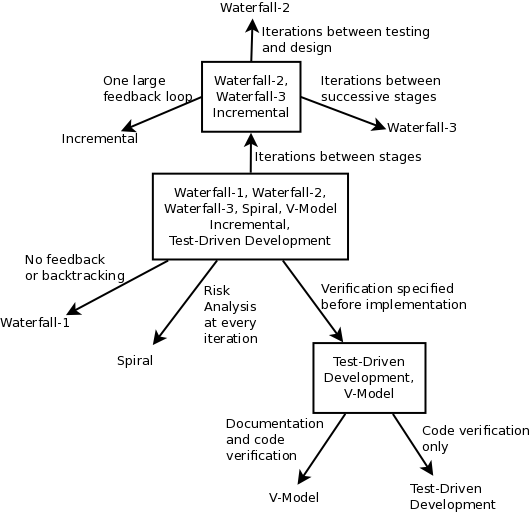
\includegraphics[scale=0.4]{media/DecisionTree4}
  \caption{This showcases the classification scheme for the models in $S_{no}$.
  We use a compressed form to show the classification of each of the models.}
  \label{DecTree4}
\end{figure}

We show a final decision tree that shows our classification scheme for each of
the models in Figure \ref{DecTreeFinal}.
It is by no means the definitive standard, and indeed it has flaws that we will
explore in the next chapter.
It serves as a baseline that could perhaps later be improved.

\begin{figure}[ht!]
  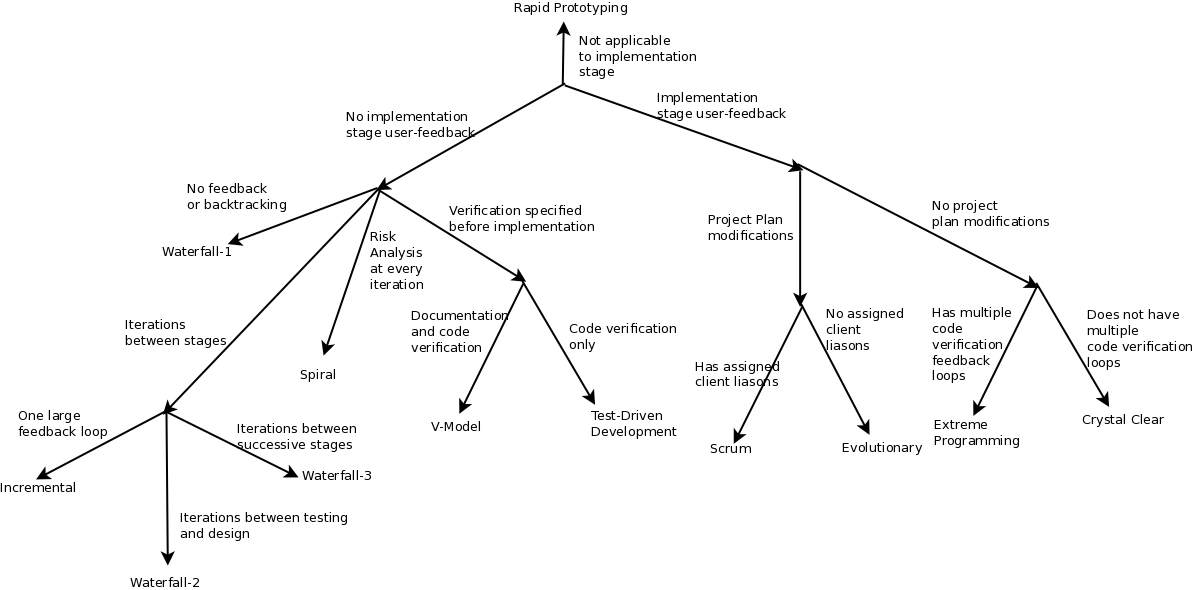
\includegraphics[angle=90,scale=0.4]{media/DecisionTreeFinal}
  \caption{Our final decision tree that we have induced. We comment on its
  accuracy, usefulness and lessons learnt in the next chapter.}
  \label{DecTreeFinal}
\end{figure}
